\documentclass[dvisvgm]{standalone}

\usepackage{tikz}
\usetikzlibrary {arrows.meta, positioning, automata}

\begin{document}

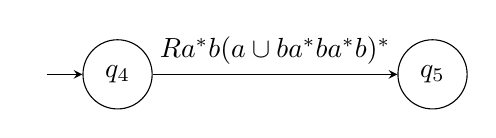
\begin{tikzpicture}[
    ->,
    >=stealth,
    node distance=4cm,
    initial text=$ $,
    on grid,
]

    \node[initial,   state]              (A) {$q_4$};
    \node[           state, right =of A] (B) {$q_5$};

    \path
        (A) edge [above]       node {$Ra^*b(a\cup ba^*ba^*b)^*$}  (B)  
    ;
\end{tikzpicture}

\end{document}